%=====================================================
%====== If you are new to LaTeX, this website ========
%======     will be your new best friend:     ========
%======   http://en.wikibooks.org/wiki/LaTeX  ========
%======   Template created by Jonathan Blair  ========
%=====================================================



%=====================================================
%============ Controls ===============================
%=====================================================

%\documentclass[12pt,letterpaper,onecolumn]{article}
\documentclass[11pt,letterpaper,onecolumn]{article}
%\documentclass[10pt,letterpaper,onecolumn]{article}  % not recommended
%\documentclass[12pt,letterpaper,twocolumn]{article}
%\documentclass[11pt,letterpaper,twocolumn]{article}
%\documentclass[10pt,letterpaper,twocolumn]{article}


\usepackage{amsmath}
\usepackage{graphicx}
\usepackage{url}
\usepackage{textgreek}
\usepackage{float}
\usepackage{booktabs}
\usepackage{subcaption}
%\graphicspath{{path-to-folder-containing-necessary-graphics}{other folder as necessary}}


%=====================================================
%============ \begin{document} =======================
%=====================================================

\begin{document}

%=====================================================
%============ Title ==================================
%=====================================================

\title{\bf Observation of the Behavior of an Operational Amplifier Oscillators}
%\title{\Large\bf Larger, Bolded Title}

%=====================================================
%============ Author =================================
%=====================================================
\author{
 Jairo Portillo \\*
  \\*
 PHY 338K Electronic Techniques \\* 
 Department of Physics \\*
 The University of Texas at Austin \\*
 Austin, TX 78712, USA
}
\date{May 6, 2016}

%\address{The University of Texas, Austin, Texas, 78712}

\maketitle

%=====================================================
%============ Abstract ===============================
%=====================================================

\begin{abstract}

In this lab, we will explore the behavior of a Operational Amplifier as a relaxation oscillator and a Wien bridge oscillator. We will observe and measure the effects of changing resistors in the relaxation oscillator and how it influences the oscillator. We will also observe how varying resistors will affect the output of the Wien bridge oscillator.
\end{abstract}

%=====================================================
%============ Body of the article ==========================
%=====================================================

%=====================================================
%============ Section ==================================
%=====================================================

\section{Preperation}

 In order to prepare for this lab, we must review the behavior of relaxation oscillator and a Wien bridge oscillator. A relaxation oscillator is made by charging a capacitor, then discharging it rapidly when the voltage reaches some threshold, beginning the cycle again. The capacitor is charged by the negative feedback loop. When a Voltage is applied, the op amp becomes positively saturation and the capacitor begins to charge $+V_{cc}$ with time constant RC. At $.5V_{cc}$, the op amp switches to negative saturation and the capacitor begins discharging toward $-V_{cc}$ with the same time constant. The time constant can be found using 
 $$\tau = 2RC\ln\left(\frac{1-x}{1+x}\right)$$
 with 
 $$ x = \frac{R_1}{R_1 + R_2}$$
 
\begin{figure}[H]
\begin{subfigure}{.5\textwidth}
  \centering
  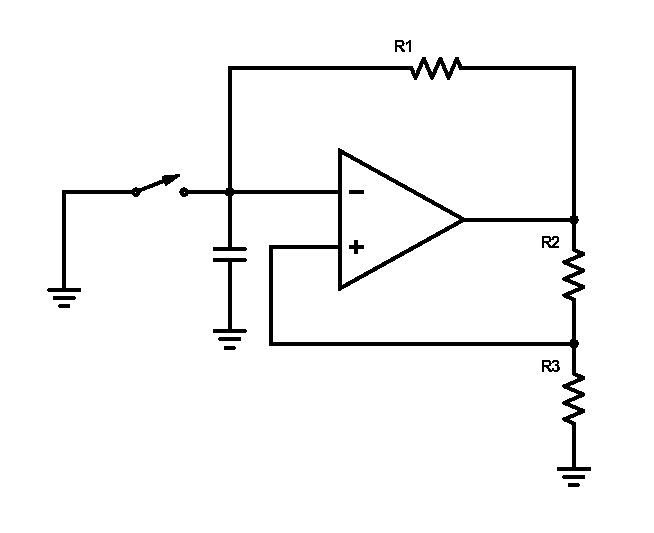
\includegraphics[scale =.6]{Lab-11-fig1.pdf}
  \caption{Relaxation Oscillator}
  \label{fig:sub1}
\end{subfigure}%
\begin{subfigure}{.5\textwidth}
  \centering
  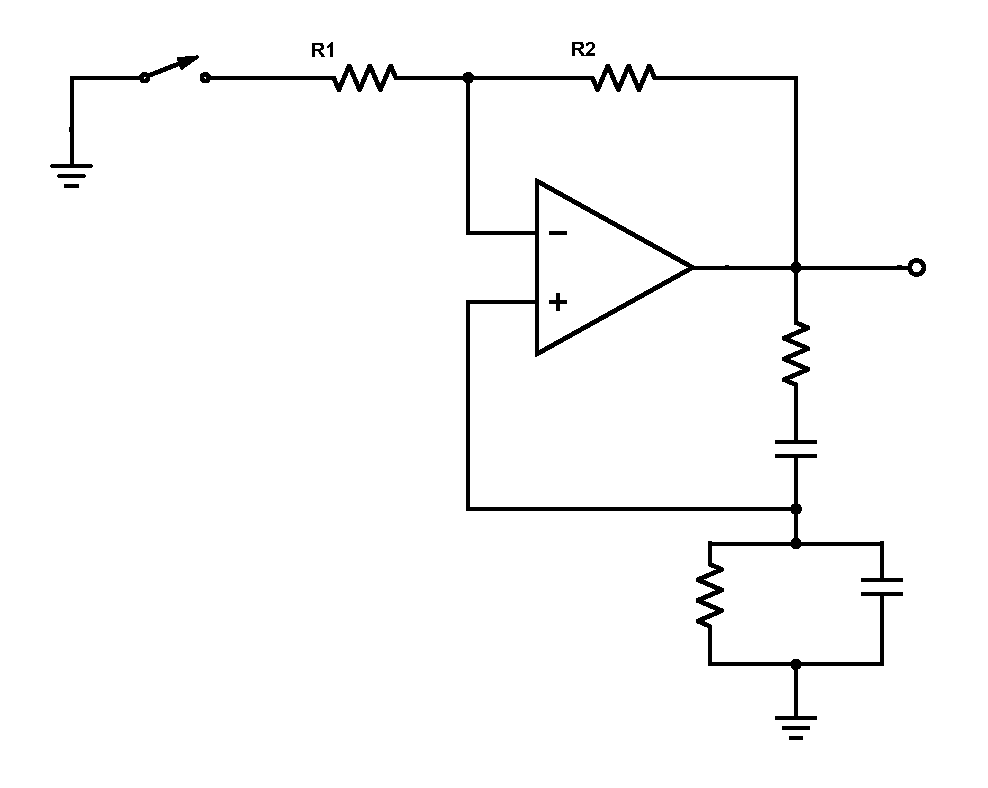
\includegraphics[scale=.5]{Lab-11-fig2.pdf}
  \caption{Wien Bridge Oscillator}
  \label{fig:sub2}
\end{subfigure}
\caption{Operational Amplifier Oscillators}
\label{fig:test}
\end{figure}

The Wien bridge oscillator is a source of low distortion sinusoidal signals at low to moderate frequencies. The oscillator is made with a feedback amplifier with no phase shift for the non inverting input and $180^{\circ}$ phase shift for the inverting input. The loop gain is then adjusted so that a self sustaining oscillation takes place. If there is more gain that the threshold gain, the output will saturate and if there is less gain, the output will cease. The period depends on the time constant of the capacitor,
$$f=\frac{1}{2\pi RC}$$
The relations of R and $R_2$ should be $2R=R_2$.

\section{Lab work}

\subsection{Data Collection}

In the relaxation oscillator, we kept R to be 10 k$\Omega$ and C to be 25 pF.The DC power supply was set to 10V and Channel 1 of the oscilloscope was connected to the output. Once the ground switch was disconnected, oscillation was observed. The peak voltage of the oscillator was found to be 9.4V. 

\begin{table}[H]
\centering
\begin{tabular}{|c|c|c|c|}
 \hline
 $R_1$ & $R_2$ & Expected & Measured \\
 $\left(\Omega \right)$ & $\left(\Omega \right)$ & $\left(kHz\right)$ & $\left(kHz\right)$ \\\hline
 50 & 100 & 2.885 & 5.482\\
 100 & 2.2 & .442 & 1.029\\
 2.2 & 100 & 46.44 & 16.55\\\hline

\end{tabular}
\caption{Results of Varying $R_1$ and $R_2$}
\label{tab:data1}
\end{table}

We can see that the closer the ratio of $\frac{R_1}{R_1 + R_2}$ was to 1 the smaller the error between the observed and expected. However it is also worth nothing that the closer the ratio was to .5, the oscillation had a more square wave shape. This was interesting as the relationship between $V_{cc}$ and $V_{out}$ is typically 
$$V_{out} = \frac{R_1}{R_1 + R_2}V_{cc}$$,
and with the maximum peak for the relaxation oscillator being $\frac{V_{cc}}{2}$, thus it can be inferred that there is a relationship of some sort between the output peak and period.

Unfortunately, the Wien bridge oscillator was unable to function even with the TA's assistance. This was likely due to internal malfunction of the op amp as various combinations of capacitors and resistors were used. The expectation for the bridge oscillator was that at high gain the output would be a square wave, at low gain the output flat lines, and that at certain ranges the output is a sine wave. 

\section{Summary and conclusions}

In this lab, we have seen how an operational amplifier can be used to form relaxation oscillator and a Wien bridge oscillators. We observed the closer the frequency was to RC and the resistor ratio was to .5, a sqaure wave would be the output. The peak of the output was also near the $V_{cc}$ which confirms the output is saturated due to the charging and discharging of the capacitor. We were unable to conclude the Wein bridge as we could not get it to function.  



%=====================================================
%============ Bibliography  ==============================
%=====================================================



%=====================================================
%============ End ====================================
%=====================================================

\end{document}

%=====================================================
%============ End ====================================
%=====================================================